%----------------------------------------------------------------------------------------
%	PACKAGES AND DOCUMENT CONFIGURATIONS
%----------------------------------------------------------------------------------------
\documentclass[11pt]{article}
\usepackage{amsmath} % Required for some math elements
\usepackage{hyperref} 
\usepackage[usenames,dvipsnames]{xcolor}
\usepackage{lipsum} 
\usepackage{cite}
\usepackage{graphicx} % Required for the inclusion of images
\usepackage{algorithmic}
\usepackage{array}
\usepackage{bookmark}
\usepackage{listings}
\usepackage{amssymb}
\usepackage{enumitem}
\usepackage[margin=24mm]{geometry}
\usepackage[caption=false, font=footnotesize]{subfig}
\usepackage{multirow}
\usepackage[active,tightpage]{preview}

\renewcommand{\PreviewBorder}{1in}
\newcommand{\Newpage}{\end{preview}\begin{preview}}

\newlist{steps}{enumerate}{1}
\setlist[steps, 1]{label = Step \arabic*:}

\hypersetup{ %color attributes of citation, link, etc.
    colorlinks=true,
    linkcolor=blue,
    filecolor=gray,      
    urlcolor=blue,
    citecolor=blue,
}

 
\lstdefinelanguage{VHDL}{
   morekeywords=[1]{
     library,use,all,entity,is,port,in,out,end,architecture,of,
     begin,and,or,Not,downto,ALL
   },
   morekeywords=[2]{
     STD_LOGIC_VECTOR,STD_LOGIC,IEEE,STD_LOGIC_1164,
     NUMERIC_STD,STD_LOGIC_ARITH,STD_LOGIC_UNSIGNED,std_logic_vector,
     std_logic
   },
   morecomment=[l]--
}
\definecolor{keyword}{rgb}{0,0.3,0.7}
\definecolor{STD}{rgb}{0.9,0.0,0.7}
\definecolor{comment}{rgb}{0.0,0.6,0.1}

\lstdefinestyle{vhdl}{
   language     = VHDL,
   basicstyle   = \footnotesize\ttfamily,
   keywordstyle = [1]\color{keyword}\bfseries,
   keywordstyle = [2]\color{STD}\bfseries,
   commentstyle = \color{comment}
   breaklines=true,                % sets automatic line breaking
   tabsize=3		                   % sets default tabsize to 2 spaces
}


\newcommand{\matlab}{\textsc{Matlab }} %very important and totally necessary addition

\newcommand\Item[1][]{%
  \ifx\relax#1\relax  \item \else \item[#1] \fi
  \abovedisplayskip=0pt\abovedisplayshortskip=0pt~\vspace*{-\baselineskip}}
  %----------------------------------------------------------------------------------------
%	DOCUMENT INFORMATION
%----------------------------------------------------------------------------------------
 
\title{ECEN302 : Integrated Digital Electronics \\ Lab 3 Submission}
\author{Daniel Eisen : 300447549}
\date{\today}

\begin{document}
\begin{preview}
\maketitle
%----------------------------------------------------------------------------------------
%	DOCUMENT CONTENT
%----------------------------------------------------------------------------------------
\section{Objectives}
This lab focuses on code reusability and packaging. It's purpose is to show and familiarise ourselves with wrapping up sections of code for multiple reuses throughout the project. These are done with Procedures and Functions; each with different specification and use cases, as well as unique restrictions.

Lastly there is an exercise in testbench development, an integral part of HDL design as it allows for the quickly modelling an implementation and extracting more internal information about the operation that can even be seen in hardware.

\section{Methodology}
  For procedures and functions the flow was to read and run a simpler provided vhdl program to confirm it functionality then to write a more complex/larger design and confirm its functionality with a provided testbench.

  In the testbench section, we are provided with an example in which be enable/explore tcl-console output and then we write our own to provide a specified output.
  \subsection{Procedures}
  Procedures are a more general purpose sub-programming construct, and allow for wrapping up practically any logical block of code for reuse. It can be sequential or combinatorial, contain delays, take any port types as arguments etc. It is simply wrapped and called later.
  \lstinputlisting[language = VHDL]{inc/calc_even_parity_procedure.vhd}

  The procedure we designed and wrote was an 8-bit parity checker that took a 8-bit input number and determined if it had even parity i.e. equal 0 and 1. Parity being represented by a 0 and non-parity a 1.

  To achieve this simply, cascading XOR operations on the neighbouring bit pairs, as shown below and implemented above.
  \begin{center}
    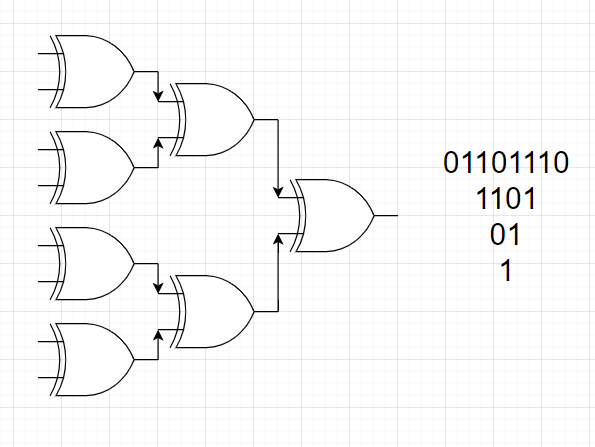
\includegraphics[width=0.49\textwidth]{inc/xor.png}
    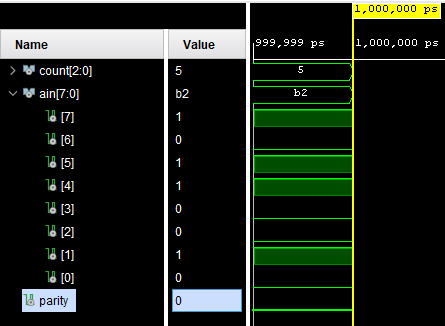
\includegraphics[width=0.49\textwidth]{inc/3_1_2.PNG}
  \end{center}
  

  \subsection{Functions}
  Functions are a more specialised method of code wrapping. Differing primary in that they can return a value directly for use, not just modifying a signal/port. More specifically they have much stricter requirements:
  The logic must be purely combinatorial, a return type must be specified, can only accept input arguments, and contain non-blocking operations.

  \lstinputlisting[language = VHDL]{inc/calc_ones_function.vhd}
  \begin{center}
    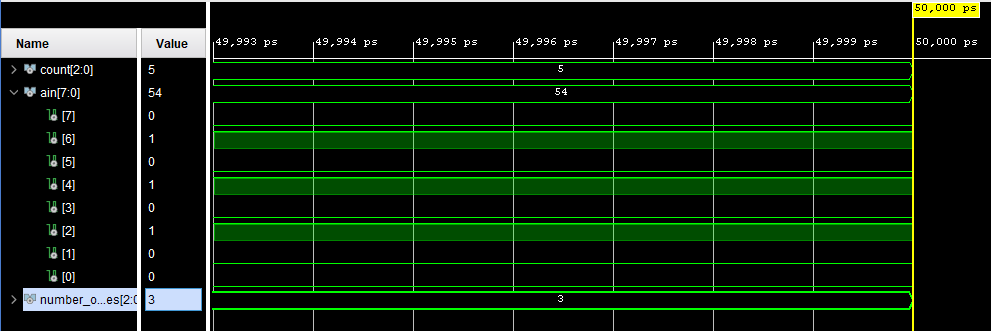
\includegraphics[width=0.67\textwidth]{inc/3_2_2.PNG}
  \end{center}

  The code and testing above, demonstrated the use of a function taking a 8 bit input and counting each bit that contains a one, and returns a 3 bit word. This is done inside a loop, and testing with the provided testbench.

  \subsection{Testbench}
  \begin{center}
    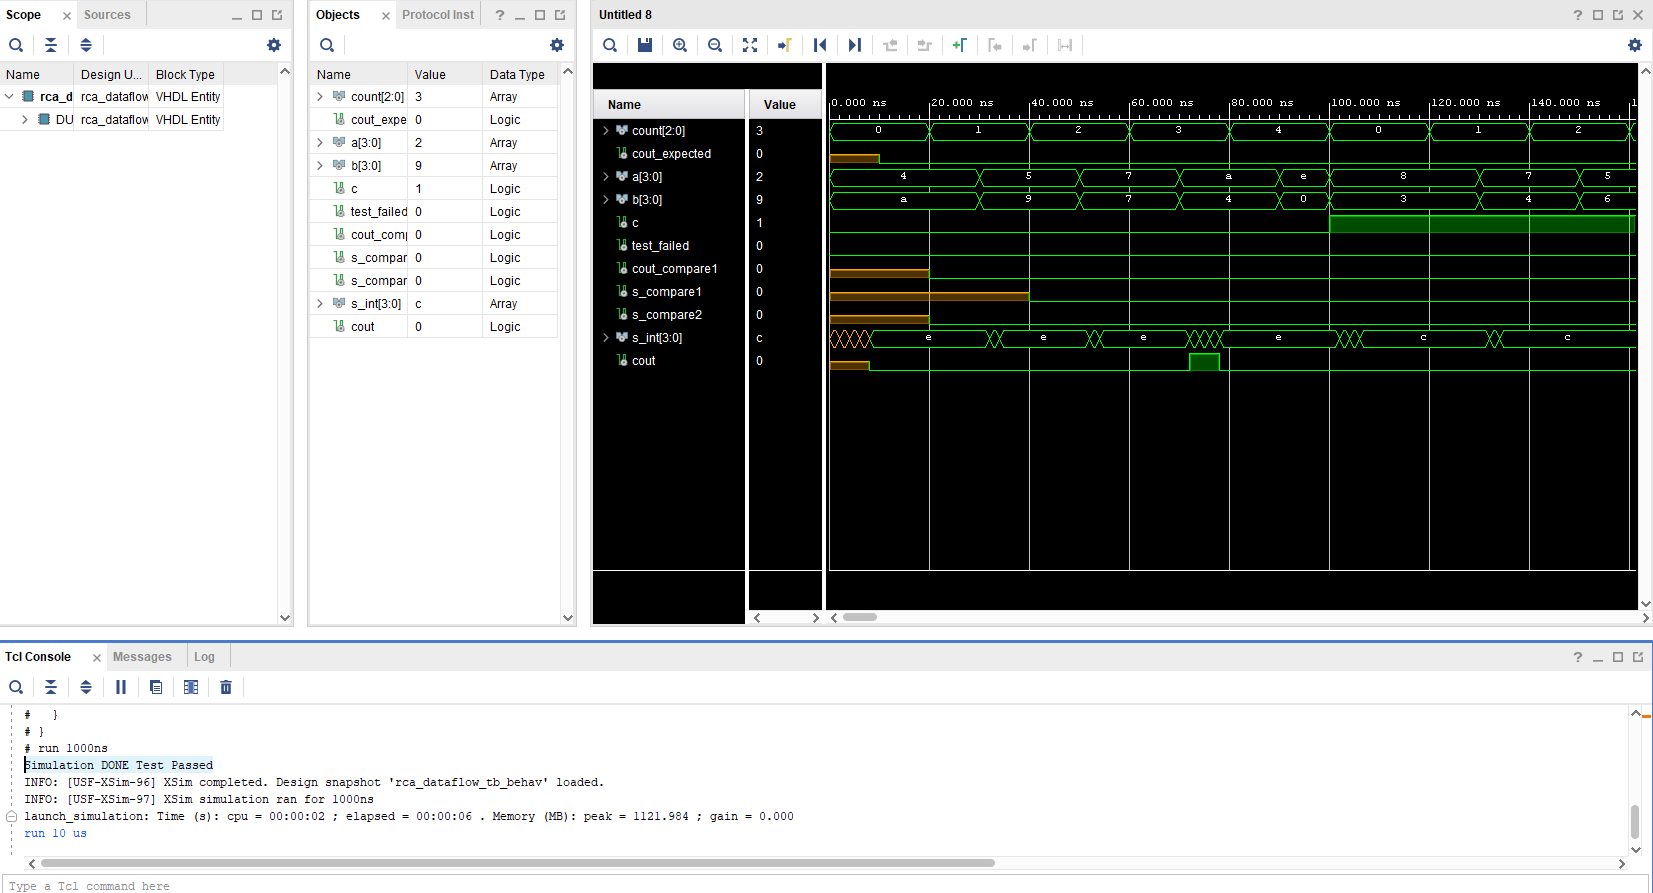
\includegraphics[width=0.67\textwidth]{inc/3_3_1.PNG}
  \end{center}

  Above shows the tcl console output writing achieved by the testbench, this required some uncommenting write calls and casting string literals as \texttt{string'}.

  \lstinputlisting[language = VHDL]{inc/waveform_generation_tb.vhd}
  \begin{center}
    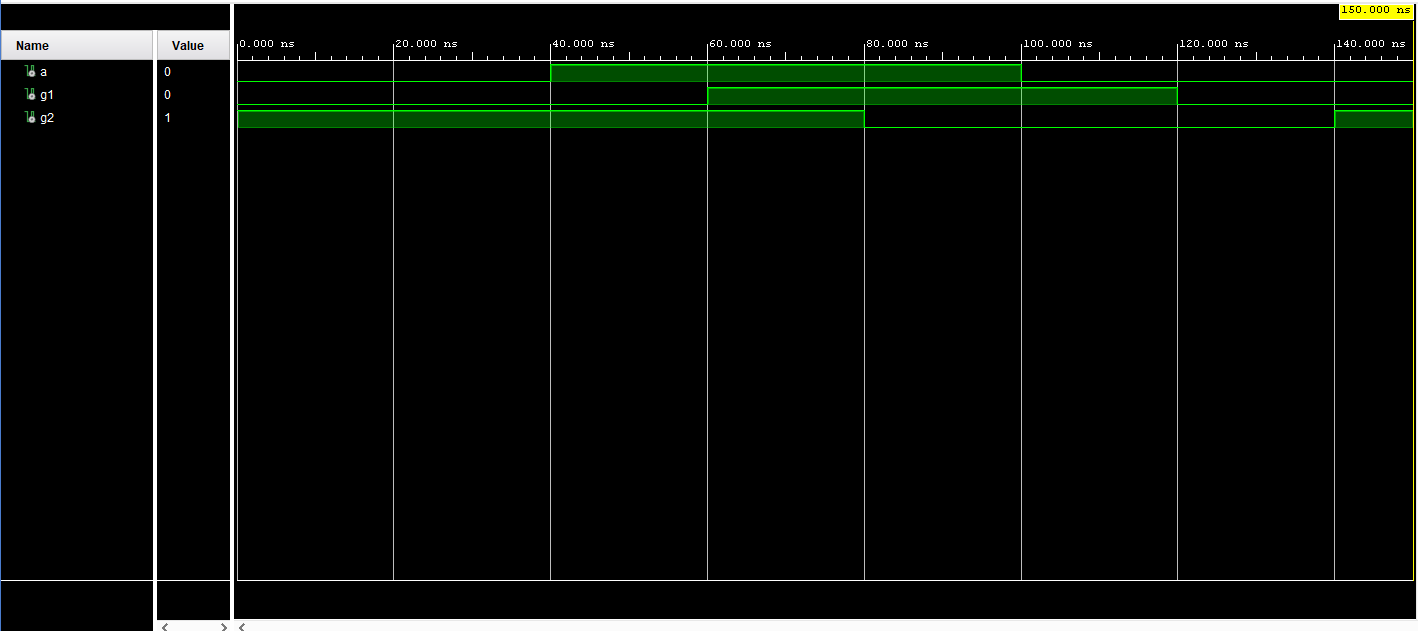
\includegraphics[width=0.67\textwidth]{inc/3_3_2.PNG}
  \end{center}

  This is testbench written to achieve the specified output. It uses wait statements for timing and simply toggles thee signal using not. 

\appendix
\end{preview}
\end{document}